\chapter{Mikrokomputer BeagleBone Black}
Projekt inżynierski został zrealizowany, w głównej części, na mikrokomputerze BeagleBone Black. Został on stworzony specjalnie z myślą o programistach OpenSource oraz tych, dla których liczy się niskie zużycie energii. Jest to oparta na procesorze AM335x ARM Cortex-A8, taktowany częstotliwością 1 GHz, płytka developerska, która została wyposażona w 512 MB pamięci RAM, 2 GB pamięci FLASH, akcelerator grafiki 3D. Posiada szereg różnych interfejsów, takich jak: HDMI, USB, Ethernet, czytnik kart microSD. BeagleBone'a można zasilać na dwa sposoby, pierwszy - poprzez kabel USB podłączony do USB (5V) albo przy użyciu zewnętrznego zasilacza, również 5V. Dla użytkownika zostały również wyprowadzone 96 pinów typu wejście/wyjście.

Na mikrokomputerze można zainstalować i ze swobodą korzystać z najpopolarniejszych dystrybucji Linuxa, np. Ubuntu, Debian, Fedora, Arch. Istnieje również możliwość uruchomienia na nim systemu Android.

\begin{figure}[h]
\centering
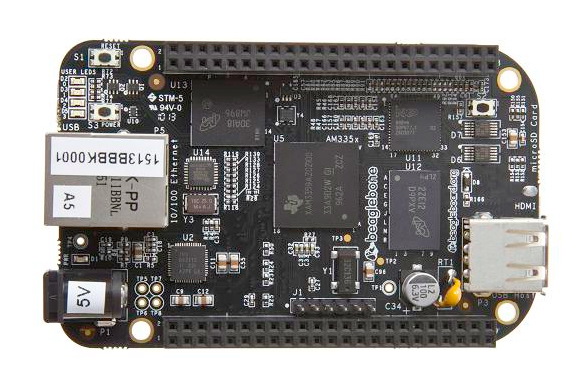
\includegraphics[scale=0.5]{beaglebone}
\caption{BeagleBone Black}
\label{fig:beaglebone}
\end{figure}

Po zakupie, domyślnie BeagleBone posiada zainstalowaną dystrybucją Linuxa - Ångström. Z uwagi na większą znajomość innego systemu operacyjnego - Ubuntu, na mikrokontrolerze została zainstalowana właśnie ta dystrybucja w wersji 13.04, dedykowana na platformę ARM Hard Float. Platforma ta posiada zaimplementowaną sprzętową obsługę liczb zmiennoprzecinkowych. Obraz systemu operacyjnego oraz instrukcję jego zainstalowania za pomocą karty pamięci microSD można znaleźć na głównej stronie projektu ARM hf: www.armhf.com.

BeagleBone został podłączony do komputera z zainstalowanym środowiskiem programistycznym przy użyciu portu USB. Po zainstalowaniu odpowiednich sterowników, które znajdują się na oficjalnej stronie producenta tej płytki oraz pamięci FLASH, port ten jest wykrywany jako interfejs sieciowy i tworzona jest sieć łącząca komputer z mikrokontrolerem. Domyślne ustawienia sprawiają, że do BeagleBone'a można podłączyć się przy użyciu protokołu SSH, łącząc się z adresem: 192.168.7.2. Po poprawnym zalogowaniu się do płytki poprzez program ssh, dostępny na Ubuntu, otrzymamy ekran podobny do tego poniżej:

\begin{figure}[h]
\centering
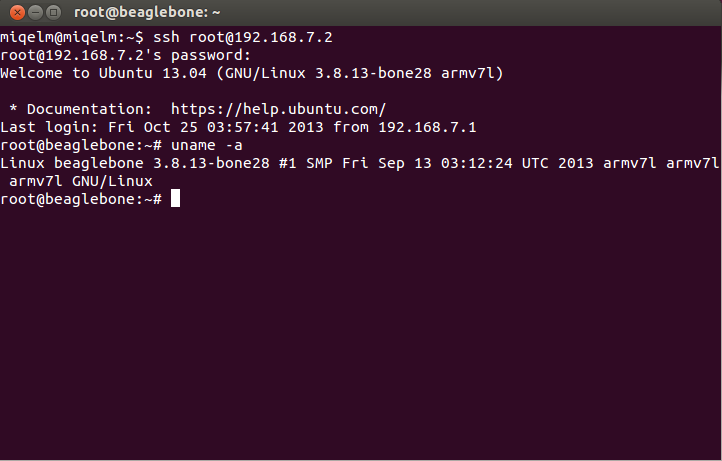
\includegraphics[scale=0.5]{konsola}
\caption{Zrzut ekranu z konsoli}
\label{fig:konsola}
\end{figure}